Using the Scenario Damage Calculator \citep{SilvaEtAl2014a} of the OpenQuake-engine, it is possible to assess the distribution of damage for a collection of assets considering a single seismic event. These results are comprised of damage per building typology, total damage distribution, and distribution of collapses in the region of interest.

\subsection{Plotting damage distribution}
\label{subsec:plot-damage_disag}
This feature of the Plotting module allows users to plot the distribution of damage across the various vulnerability classes, as well as to the total damage distribution. For what concerns the former result, it is necessary to set the path to the output file using the parameter \verb=tax_dmg_dist_file=. It is also possible to specify which vulnerability classes should be considered, using the parameter \verb=taxonomy_list=. However, if a user wishes to consider all of the vulberability classes, then this parameter should be left empty. It is also possible to specify is a 3D plot containing all of the vulnerability classes should be generated, or a instead a 2D plot per vulnerability class. For follow the former option, the parameter \verb=plot_3d= should be set to \verb=True=. It is important to understand that this option leads to a plot of damage fractions for each vulnerability class, instead of the number of assets in each damage state. An example of this output is illustrated in Figure \ref{fig:damage_disag}.

\begin{figure}[htb]
  \centering
      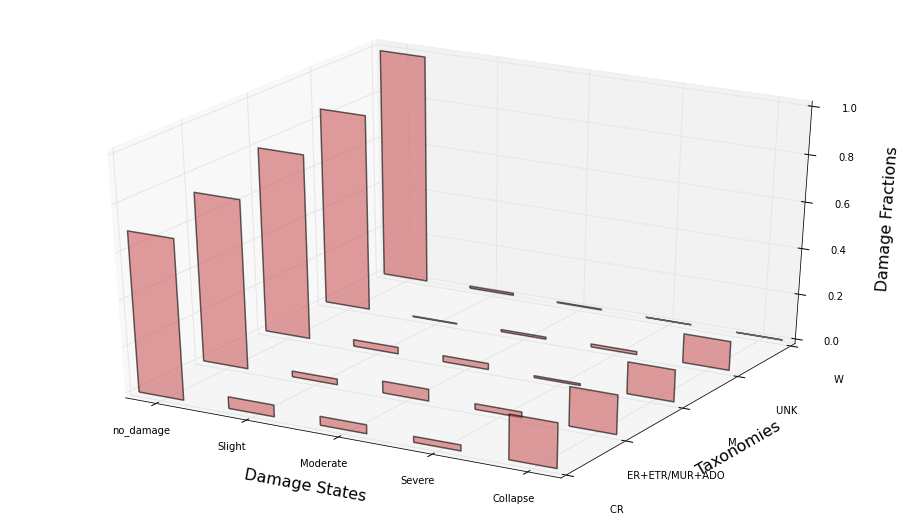
\includegraphics[width=10cm]{Figures/damage_distribution.png}
  \caption{Damage disaggregation per vulnerability class.}
  \label{fig:damage_disag}
\end{figure}

In order to plot the total damage distribution (considering the entire colection of assets), it is necessary to use the parameter \verb=total_dmg_dist_file= to define the path to the respective output file.Figure \ref{fig:total_dmg} presents an example of this type of output.

\begin{figure}[htb]
  \centering
      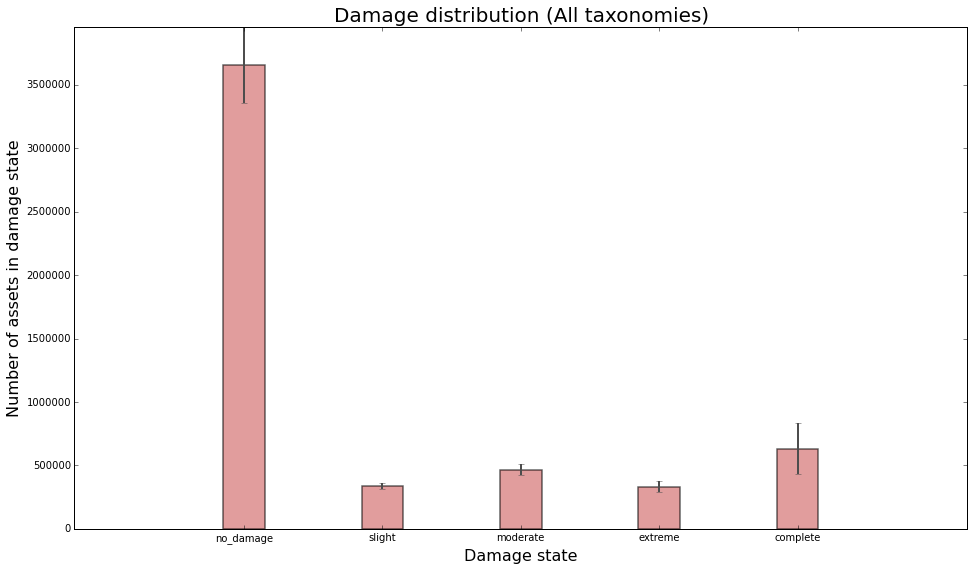
\includegraphics[width=8cm]{Figures/total_damage_dist.png}
  \caption{Total damage distribution.}
  \label{fig:total_dmg}
\end{figure}

\subsection{Plotting collapse maps}
\label{subsec:plot-collapse_maps}

The OpenQuake-engine also generates an output defining the spatial distribution of the mean (and associated standard deviation) of assets in the last damage state (usually representing collapse or complete damage). The location of this output needs to be specified using the parameter \verb=collapse_map=. Then, it is necessary to specify whether the user desires a map with the aggregated number of collapses (i.e. at each location, the mean number of collapses across all of the vulnerability classes are summed) or a map for each vulnerability class. Thus, the following options are permitted:\\

\begin{enumerate}
\item Aggregated collapse map only.
\item Collapse maps per taxonomy only.
\item Both aggregated and taxonomy-based.\\
\end{enumerate}

The plotting option should be specified using the parameter \verb=plotting_type=, and the location of the exposure model used to perform the calculations must be defined using the variable \verb=exposure_model=. A number of other parameters can also be adjusted to modify the style of the resulting collapse map as follows:\\

\begin{itemize}
\item \verb=bounding_box=: If set to 0, the Plotting module will calculate the geographical distribution of the assets, and adjust the limits of the map accordingly. Alternatively, a user can also specify the minimum/maximum latitude and longitude that should be used i nthe creation of the map.
\item \verb=marker_size=: This attribute can be used to adjust the size of the markers in the map.
\item \verb=log_scale=: If set to \verb=True=, it will apply a logarithmic scale on the color scheme of the map, pottentially allowing a better visualization of the variation of the numbers of collapses in the region of interest.\\
\end{itemize}

An example of a collapse map is presented in Figure \ref{fig:collapse_map}.

\begin{figure}[htb]
  \centering
      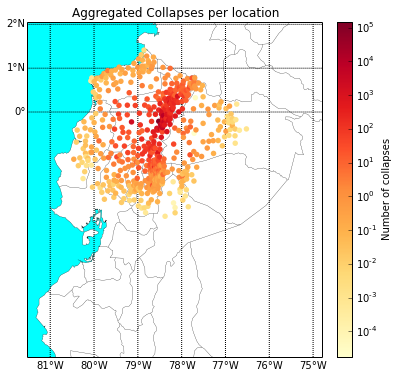
\includegraphics[width=8cm]{Figures/collapse_map.png}
  \caption{Spatial distribution of the mean number of collapses.}
  \label{fig:collapse_map}
\end{figure}
